\section{Filtering the test signal for directionality measurement}\label{sec:signal_filtering}
For the sake of simplicity, when investigating the directional characteristics of a speaker array as described in \autoref{ax:directional_3}, the filtering is done offline and the measurement routine is fed different signals as reference and outputs. These are achieved by generating a sweep in MATLAB and then using the \texttt{filter} function. The resulting signals are stored as wave files and are therefore normed so that there is no value bigger then 1.
The upper envelope of the sweep time signals is illustrated in \autoref{fig:time_signals}.
\begin{figure}[H]
	\centering
	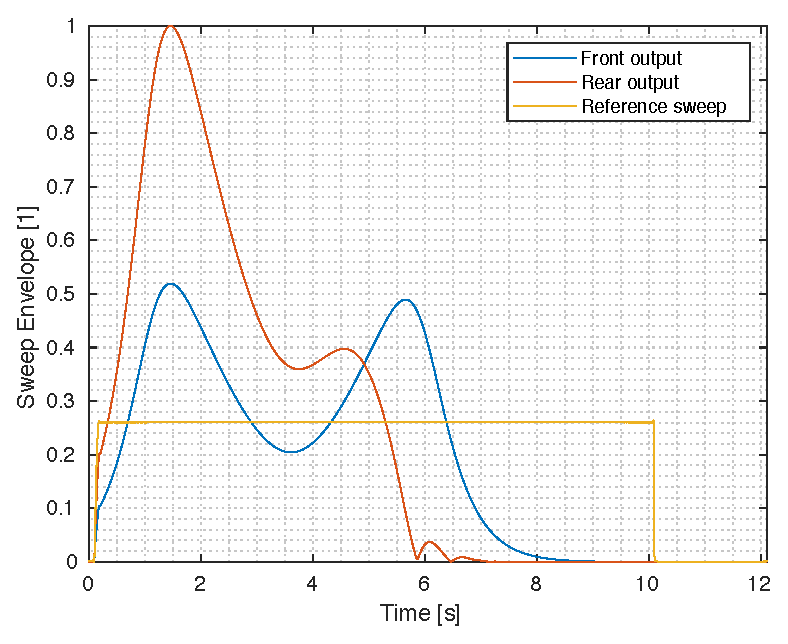
\includegraphics[width=0.7\textwidth]{time_signals.eps}
	\caption{Upper envelope of sweeps for array polar response measurement}
		\label{fig:time_signal}
\end{figure}